\documentclass[12pt]{article}
\setlength\parindent{0pt}
\usepackage{fullpage}
%\usepackage[margin=0.5in, paperwidth=13.5in, paperheight=8.4375in]{geometry}
\usepackage[margin=0.5in, paperwidth=8.5in, paperheight=11in]{geometry}

\usepackage{amsmath}
\usepackage{graphicx}
\newcommand{\BI}{\begin{itemize}}
\newcommand{\insp}{\vspace{1in}}
\newcommand{\EI}{\end{itemize}}
\newcommand{\BE}{\begin{enumerate}}
\newcommand{\EE}{\end{enumerate}}
\newcommand{\BS}{\bigskip}
\setlength{\parskip}{4mm}


\pagenumbering{gobble}

\begin{document}
	\begin{center}\sc \Large Tutorial -- The Motion of the Celestial Sphere 
		

\small

	\it 

Up the dome of heaven \\
Like a great hill \\
I watch them marching \\ 
Stately and still \\


\BS

\begin{flushright} \rm --Excerpted from ``Stars'' by Sara Teasdale (1930) \end{flushright}

\end{center}

	\normalsize
	
	{\bf Note and Foreword:} The most difficult part about this material for students is the fact that we too often study from things printed on paper or displayed on screens. These are two-dimensional, but the world is {\it three dimensional}. These exercises are designed to help you think three-dimensionally. But, until we have holographic projectors rather than paper, we have to print it for you.
	
	The {\it absolute best thing you can do} in learning this material is to put your paper down, stand up, and imagine the motion of the stars on the walls and ceiling around you, and use your fingers to point at imaginary stars as they go by. If you do this, the first quiz will likely be quite easy; if you do not, it will likely be very difficult.
	
	Note that your first homework assignment is the last page of this handout.
	

	\section{Directions in the Sky}
	
	The poet above compared the view of the night sky seen from Earth to a ``dome''. Many of us are familiar with the Dome Formerly Known As Carrier: half of a sphere, seen from the inside.
	
	We don't have a smooth sphere, but the roof of our auditorium is close enough. Before we can figure out how stars move in our sky, we will need some language to describe where things are located in the sky. 
	
	We have the familiar words {\bf north}, {\bf south}, {\bf east}, and {\bf west} to describe directions on the surface of the Earth. But, since we are describing things in the sky, we will also need the directions {\bf up} and {\bf down}, or {\bf above} and {\bf below}.
	
	Since {\bf up} and {\bf down} are relative, you can relate them to your eye level, or the {\bf horizontal}. So you can say, for instance, things like {\it a little bit above eye level to the east}, or {\it very far up, straight overhead}, or {\it high in the sky to the southwest}.
	
	In general, to describe where something is in the sky, you need two pieces of information:
	
	\begin{enumerate}
		\item Its {\bf azimuth}: Whether it is north, south, east, or west (or somewhere in between)
		\item Its {\bf altitude}: Whether it is horizontal with you (at eye level), up, or down
	\end{enumerate}
		\newpage
	We've projected four laser-pointer dots around the room. Using this language, describe where they are. (Pretend that they are stars in the sky.) You'll want to use some words to describe both altitude and azimuth.
	
		
	\begin{enumerate}
		\item The green dot on the right-hand wall

\BS\BS\BS
		
		\item The green dot on the ceiling
	
	\BS\BS\BS	
		\item The red dot on the floor in front of the room
\BS\BS\BS

		
		\item The red dot on the projection screen
\BS\BS\BS
		
	\end{enumerate}


\subsection{The Horizontal and the Horizon}

We can see things below the horizontal (below our eye level) very easily in this room, including some of the laser dots. Astronomers use the word {\it horizon} to describe their ``horizontal'' wherever they are on Earth's surface. 

If we are standing on Earth's surface, can we see stars below ``eye level'', the ``horizontal'', or the ``horizon''? (These words all mean the same thing.) Why or why not?

\insp



\section{The Motion of the Celestial Sphere}

As we saw in the video from the Quad, the stars move as though they are attached to a sphere rotating around Earth, once per day. There is a bright star, the {\it North Star} or {\it Polaris}, near the axis of this sphere that doesn't move much at all. The white line runs from Earth to the North Star.

How would you describe where Polaris is in the sky, using the language of the last section?

\BS\BS\BS\BS

\newpage

\begin{minipage}{0.4\textwidth}
We now have a way to represent where things are in the real sky in {\it words}. But we also need a way to do it in diagrams. This is hard, since our sky is three-dimensional but our paper is flat. We can represent the sky above our heads on a circular diagram, though, as shown on the right.

\bigskip

In this diagram, the zenith (above our heads) is at the center, and the horizon is the outer ring. Note that North is on the right; this makes the directions line up with the real directions if you are sitting in Stolkin Auditorium facing forward.

\end{minipage}
\begin{minipage}{0.6\textwidth}
	\begin{center}
		\large Sky Above Us\\
		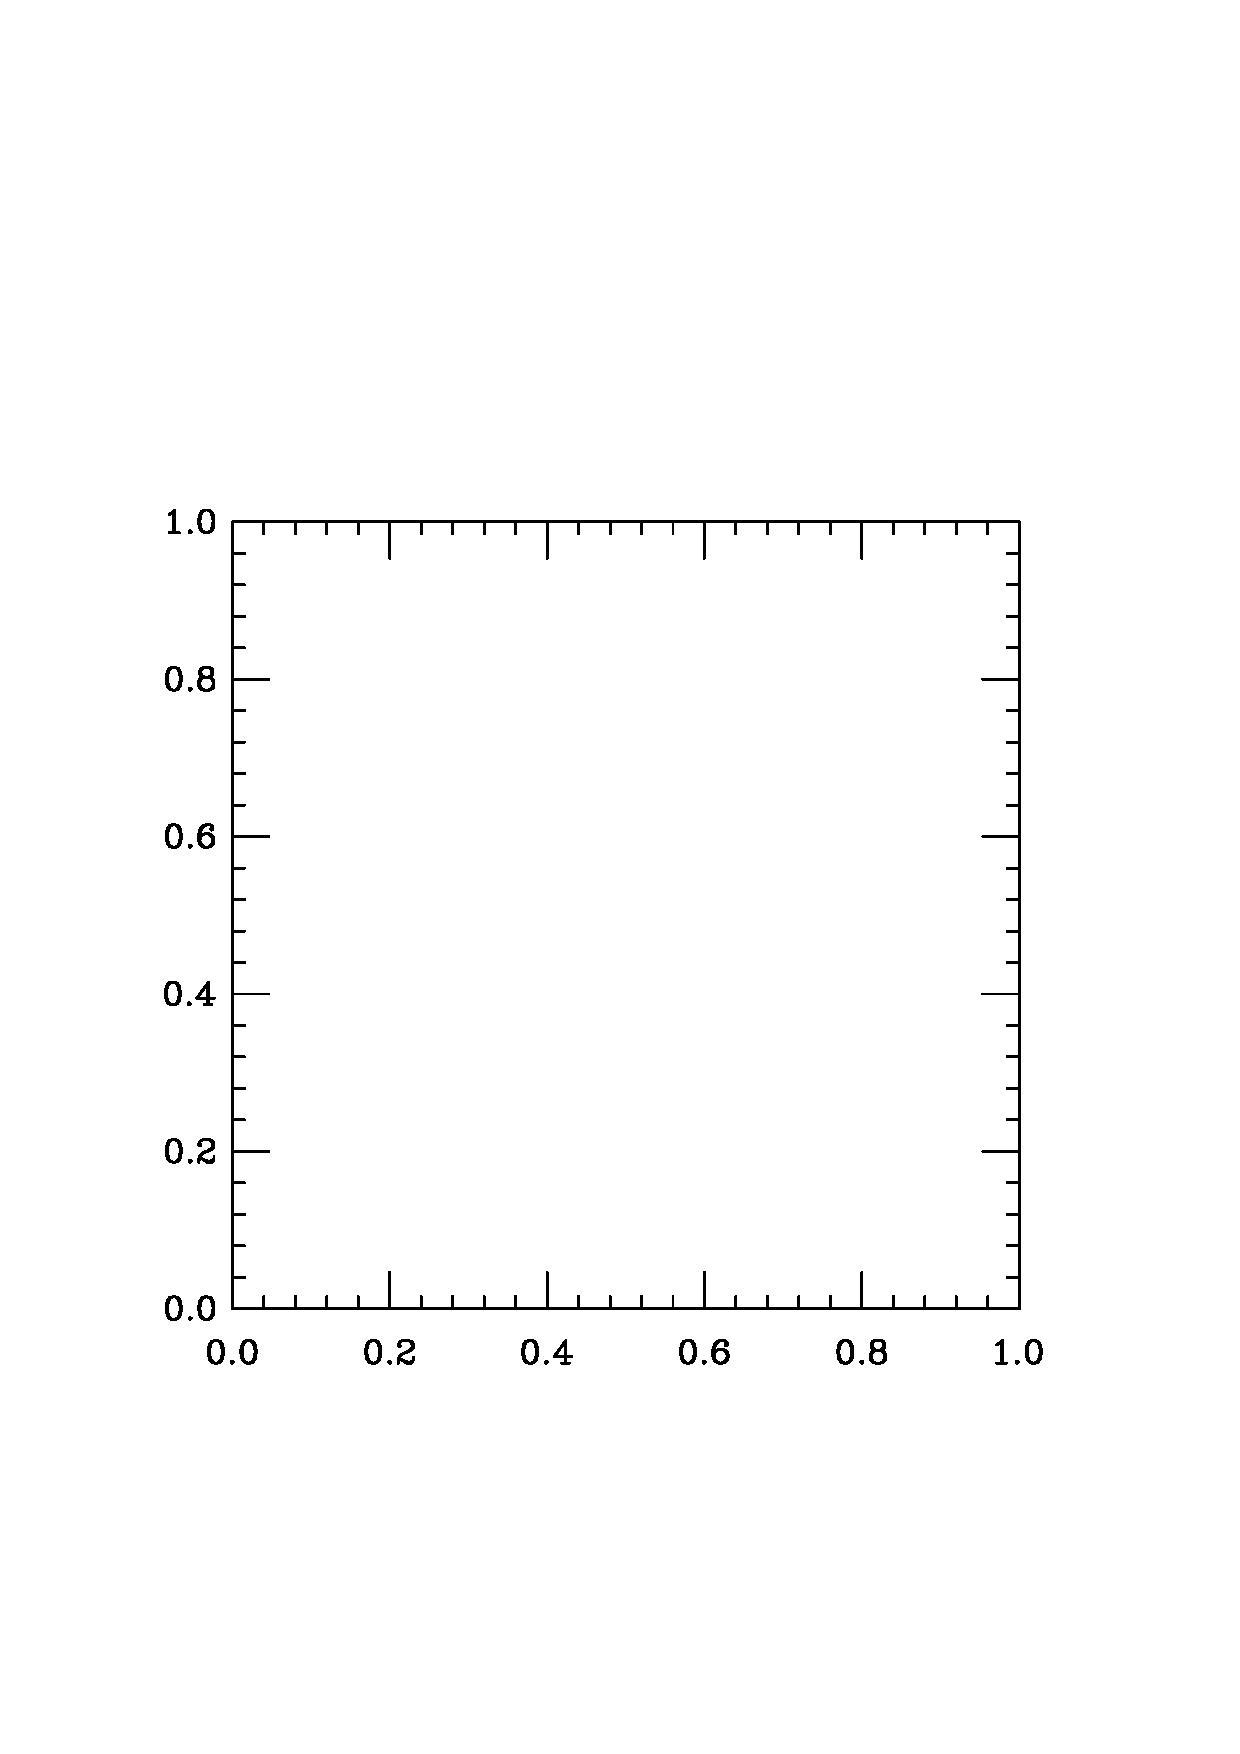
\includegraphics[width=0.8\textwidth]{topsky-crop.pdf}
	\end{center}
\end{minipage}




In the video from the Quad, we saw that one star in the northern sky doesn't move very much: Polaris, located halfway between the northern horizon and the zenith, at the North Celestial Pole. Point to it with your finger (in the real world, in the auditorium!). Then mark where it is with a $\star$ and label it in your diagram.

\insp

Now, let's figure out how things move.

At midnight, the star Dubhe will be low in the sky, just above the northern horizon. Label this point on your diagram above, then point to it in the real world. (If you are not sure, as always, talk to the people around you, or ask us for help!)

\vspace{0.7in}

We saw from the Quad video that all of the stars move in a counterclockwise circle around the North Celestial Pole, near Polaris. Dubhe will do this too, so draw the path that Dubhe will follow over one day on your diagram. Then, using your finger, trace the path that Dubhe makes in the real world. Will it ever reach the zenith? Will it get close?

\vspace{0.7in}

We know that stars make one complete circle around the North Celestial Pole in one day. We know where Dubhe will be at midnight... but where will it be later in the day? Label the positions of Dubhe at 3 AM, at 6 AM, at 9 AM, and at 6 PM on your diagram, then find them in the ``real sky''.

\vspace{0.7in}

As you saw earlier, Dubhe will get close to the zenith. What time will this happen? Will you be able to see it then?

\vspace{0.7in}

Find someone next to you (hopefully one of the people you've been working with the whole time!) One of you should describe in words and by pointing their finger how Dubhe moves from midnight to noon; the other person should take over and describe how Dubhe moves from noon to midnight. 

\subsection{Rising and Setting}

Does Dubhe ever rise and set, or does it stay below the horizon all the time? How do you know?

\insp

Let's think about another star now. The bright star Altair will be high in the southern sky tonight at midnight. As with the other stars, it moves in a circle around Polaris. However, {\it this time}, that entire circle isn't above the horizon.

With your classmates, stand up and point in the real sky with your finger, tracing the path of Altair during one day. Note that it should go below the horizontal for a little while!

Then, draw that path on your diagram. Notice that now we have two diagrams, since we're thinking about rising and setting! The ``nadir'', appearing on the diagram below the horizon, is the point directly beneath our feet, opposite the zenith.


\begin{minipage}{0.5\textwidth}
\begin{center}
	\large Sky Above Horizon\\
	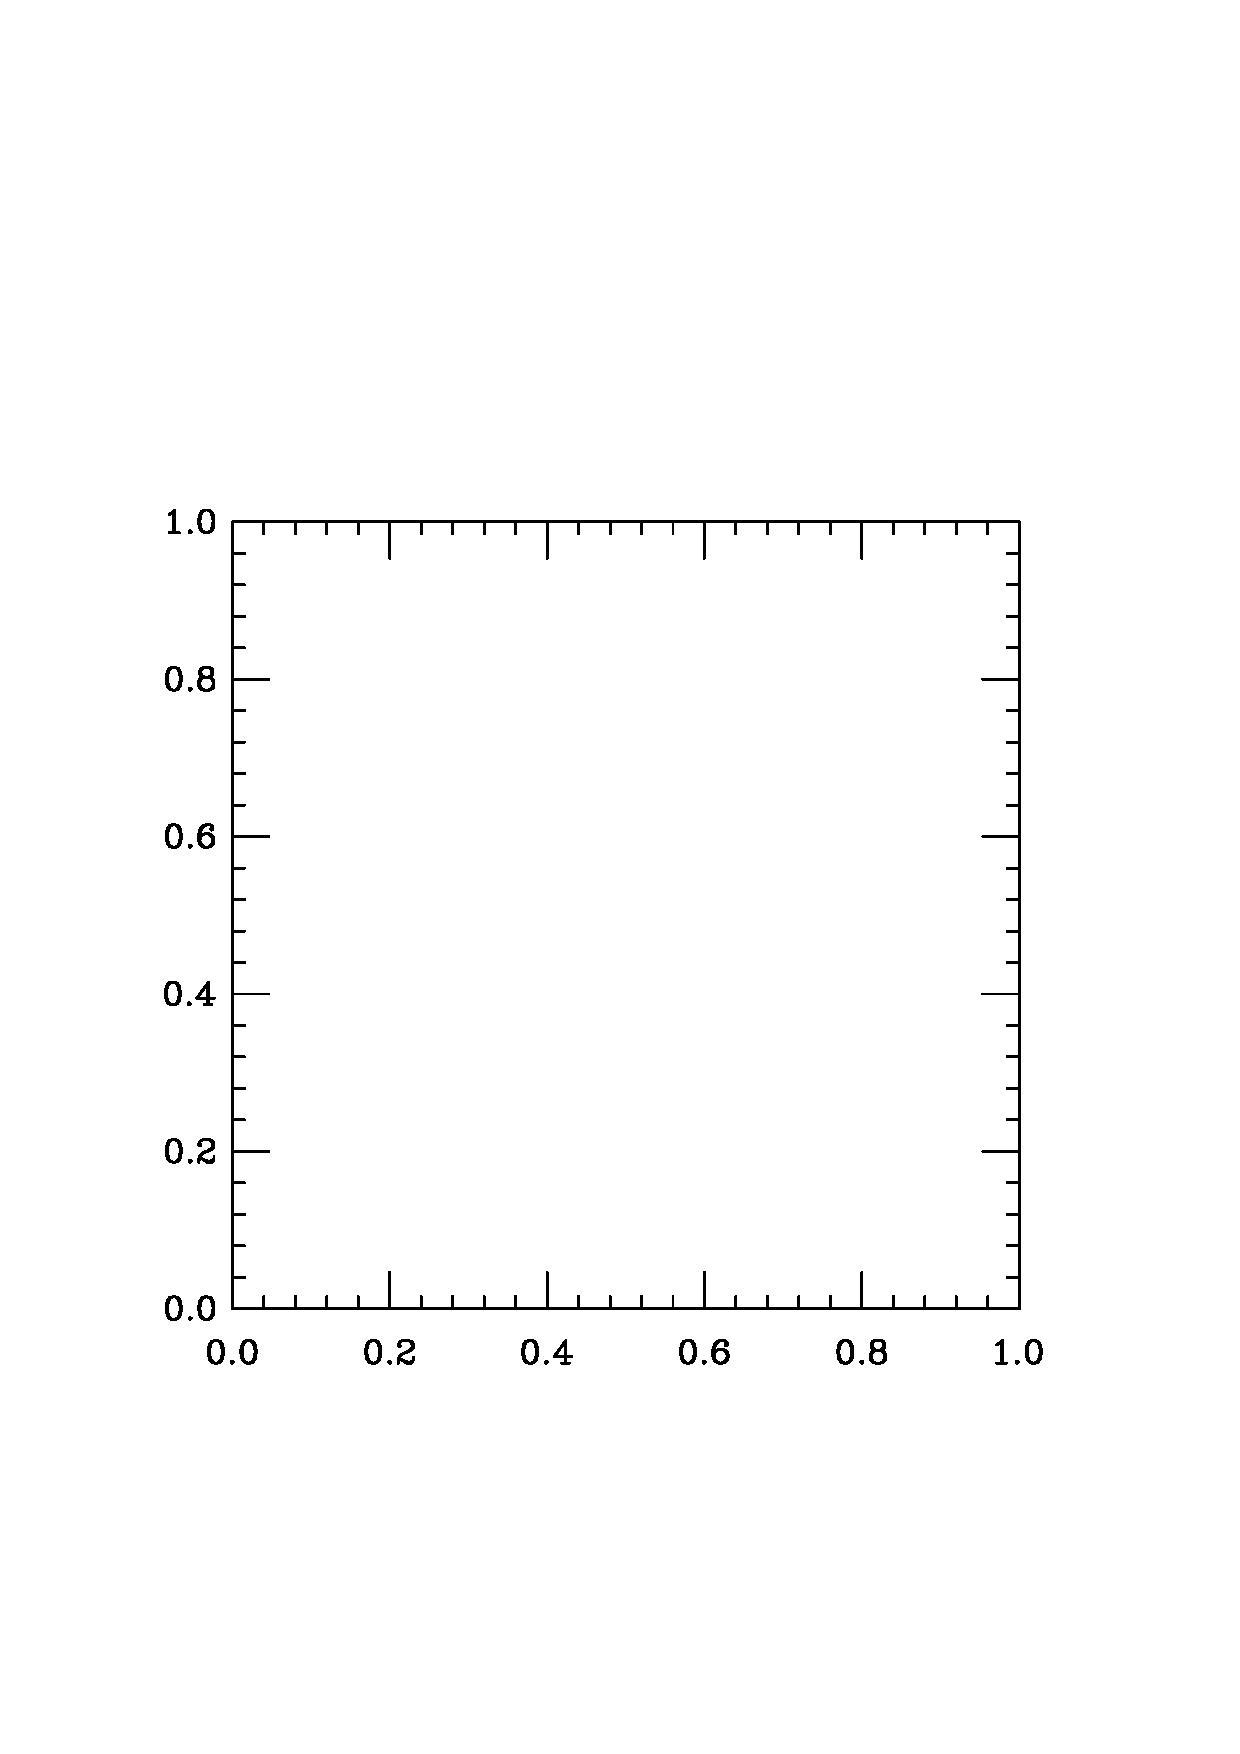
\includegraphics[width=0.8\textwidth]{topsky-crop.pdf}
\end{center}
\end{minipage}
\begin{minipage}{0.5\textwidth}
	\begin{center}
		\large Sky Below Horizon\\
		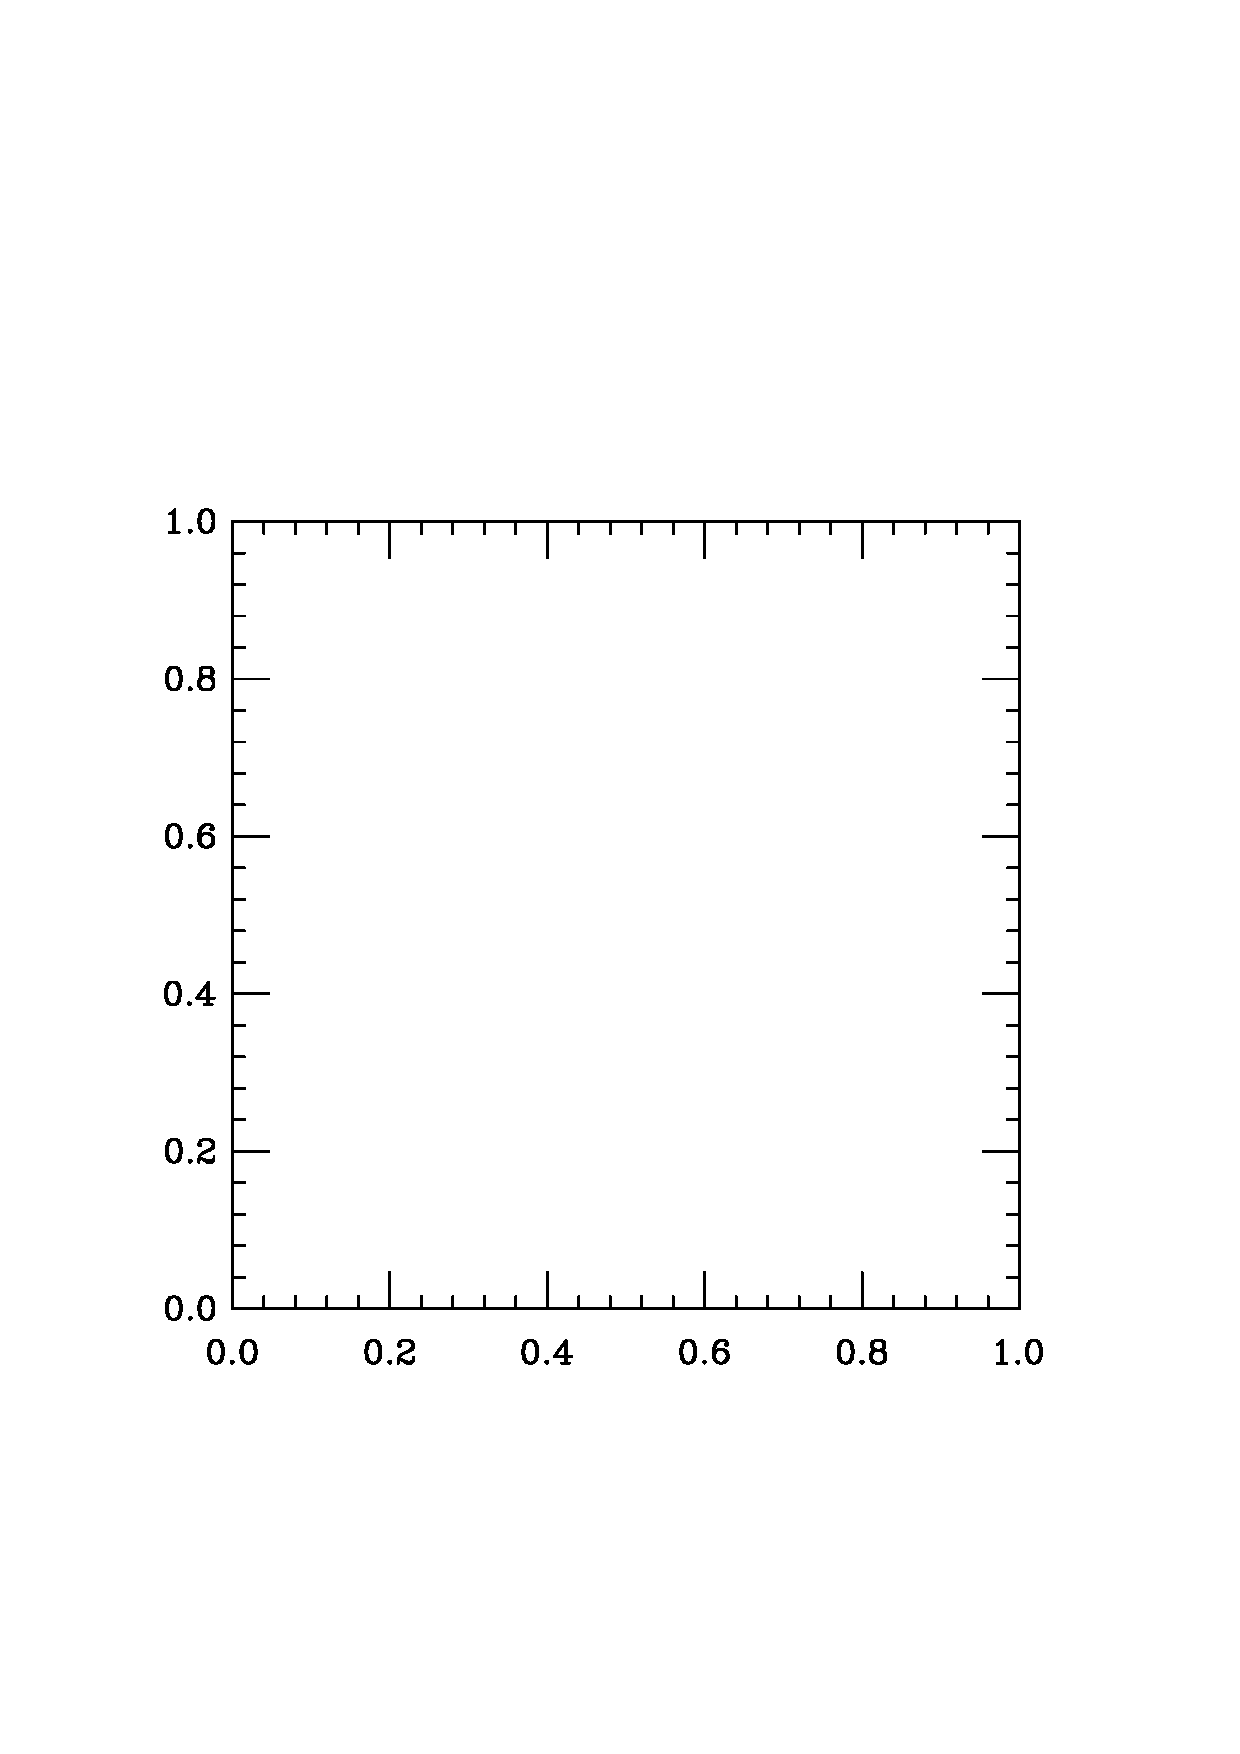
\includegraphics[width=0.8\textwidth]{botsky-crop.pdf}
	\end{center}
\end{minipage}


\section{The Sky Elsewhere}

Astronomers have known for thousands of years that the position of the North Celestial Pole depends on your location on Earth. Specifically, its altitude above the horizon is equal to how far you are north of the Equator.




The city of Helsinki, Finland is at $65^\circ$ N latitude. Here is another copy of our diagrams. Draw the position of the North Celestial Pole as seen from Helsinki. {\it (For reference, the line marked ``High in sky'' is at 60 degrees altitude.)} Then do the same for the city of Kampala, Uganda, which is located near the Equator. 


\begin{minipage}{0.5\textwidth}
	\begin{center}
		\large Sky Above Horizon\\
		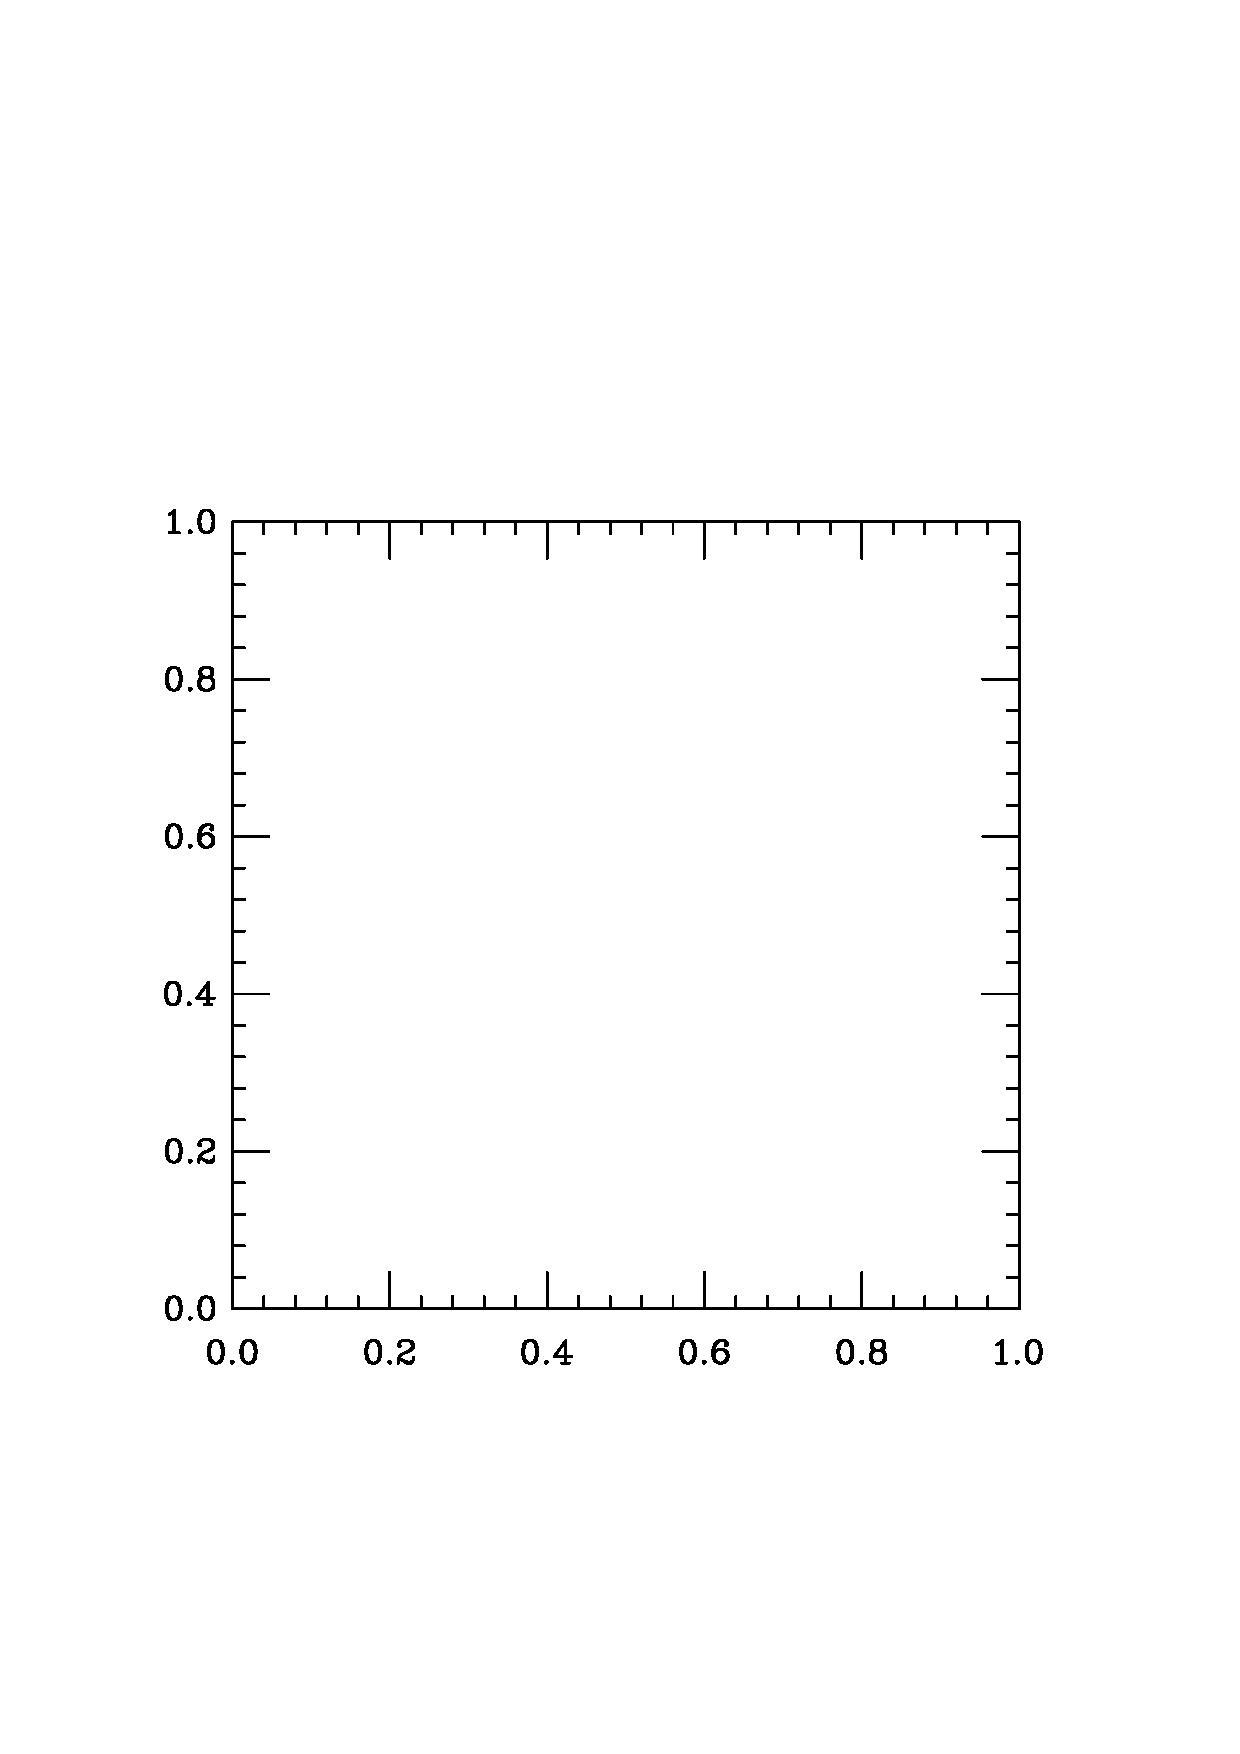
\includegraphics[width=0.75\textwidth]{topsky-crop.pdf}
	\end{center}
\end{minipage}
\begin{minipage}{0.5\textwidth}
	\begin{center}
		\large Sky Below Horizon\\
		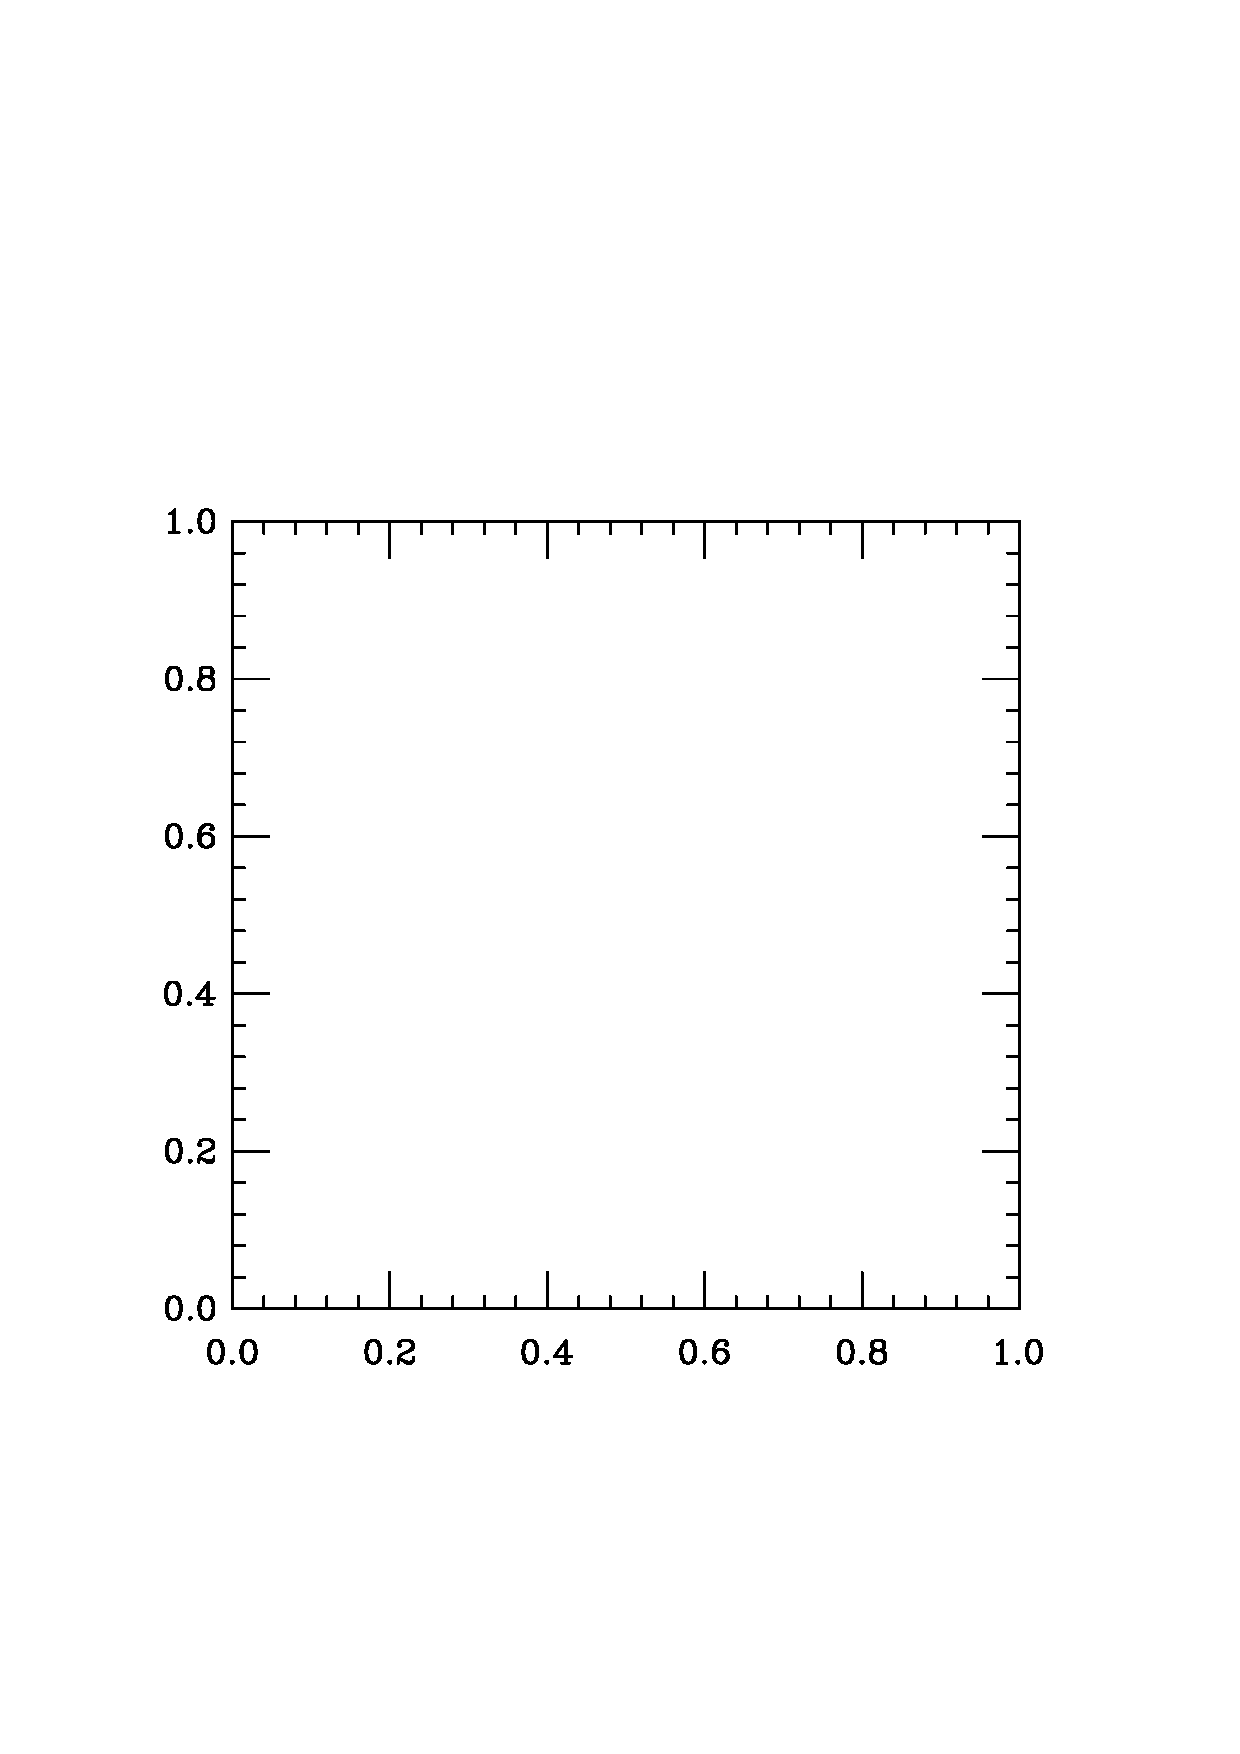
\includegraphics[width=0.75\textwidth]{botsky-crop.pdf}
	\end{center}
\end{minipage}
\bigskip

The star Kochab is located pretty close to Polaris. Draw the path that Kochab makes in the sky as seen from Helsinki and from Kampala. (Use the diagrams above for both.)

\insp

Two ancient astronomers, an Inuit (from extremely high latitudes, near the North Pole) and a Polynesian (from low latitudes, near the Equator) are describing how they see the stars move. {\it (For simplicity, suppose the Inuit has actually traveled to the North Pole, and the Polynesian is at the Equator.)}

{\bf Astronomer A:} All of the stars rise in the East and set in the West. Some of them are in the northern sky, some are in the southern sky, some are in the middle, but all of them rise and set.

{\bf Astronomer B:} I see something different. All of my stars seem to be going in a circle. They don't really rise and set; they just circle around the zenith. 

\bigskip

Which is the Polynesian and which is the Inuit, and how do you know?


\newpage

\section{The Sun as a star}

The Sun moves in the sky just like the other stars. We know from experience that the Sun rises in the East and sets in the West... but what does it do for the rest of the day? Draw the path of the Sun below. (Note that since the Sun rises and sets, it will go below the horizon at night, so you will need both diagrams.)



\begin{minipage}{0.5\textwidth}
	\begin{center}
		\large Sky Above Horizon\\
		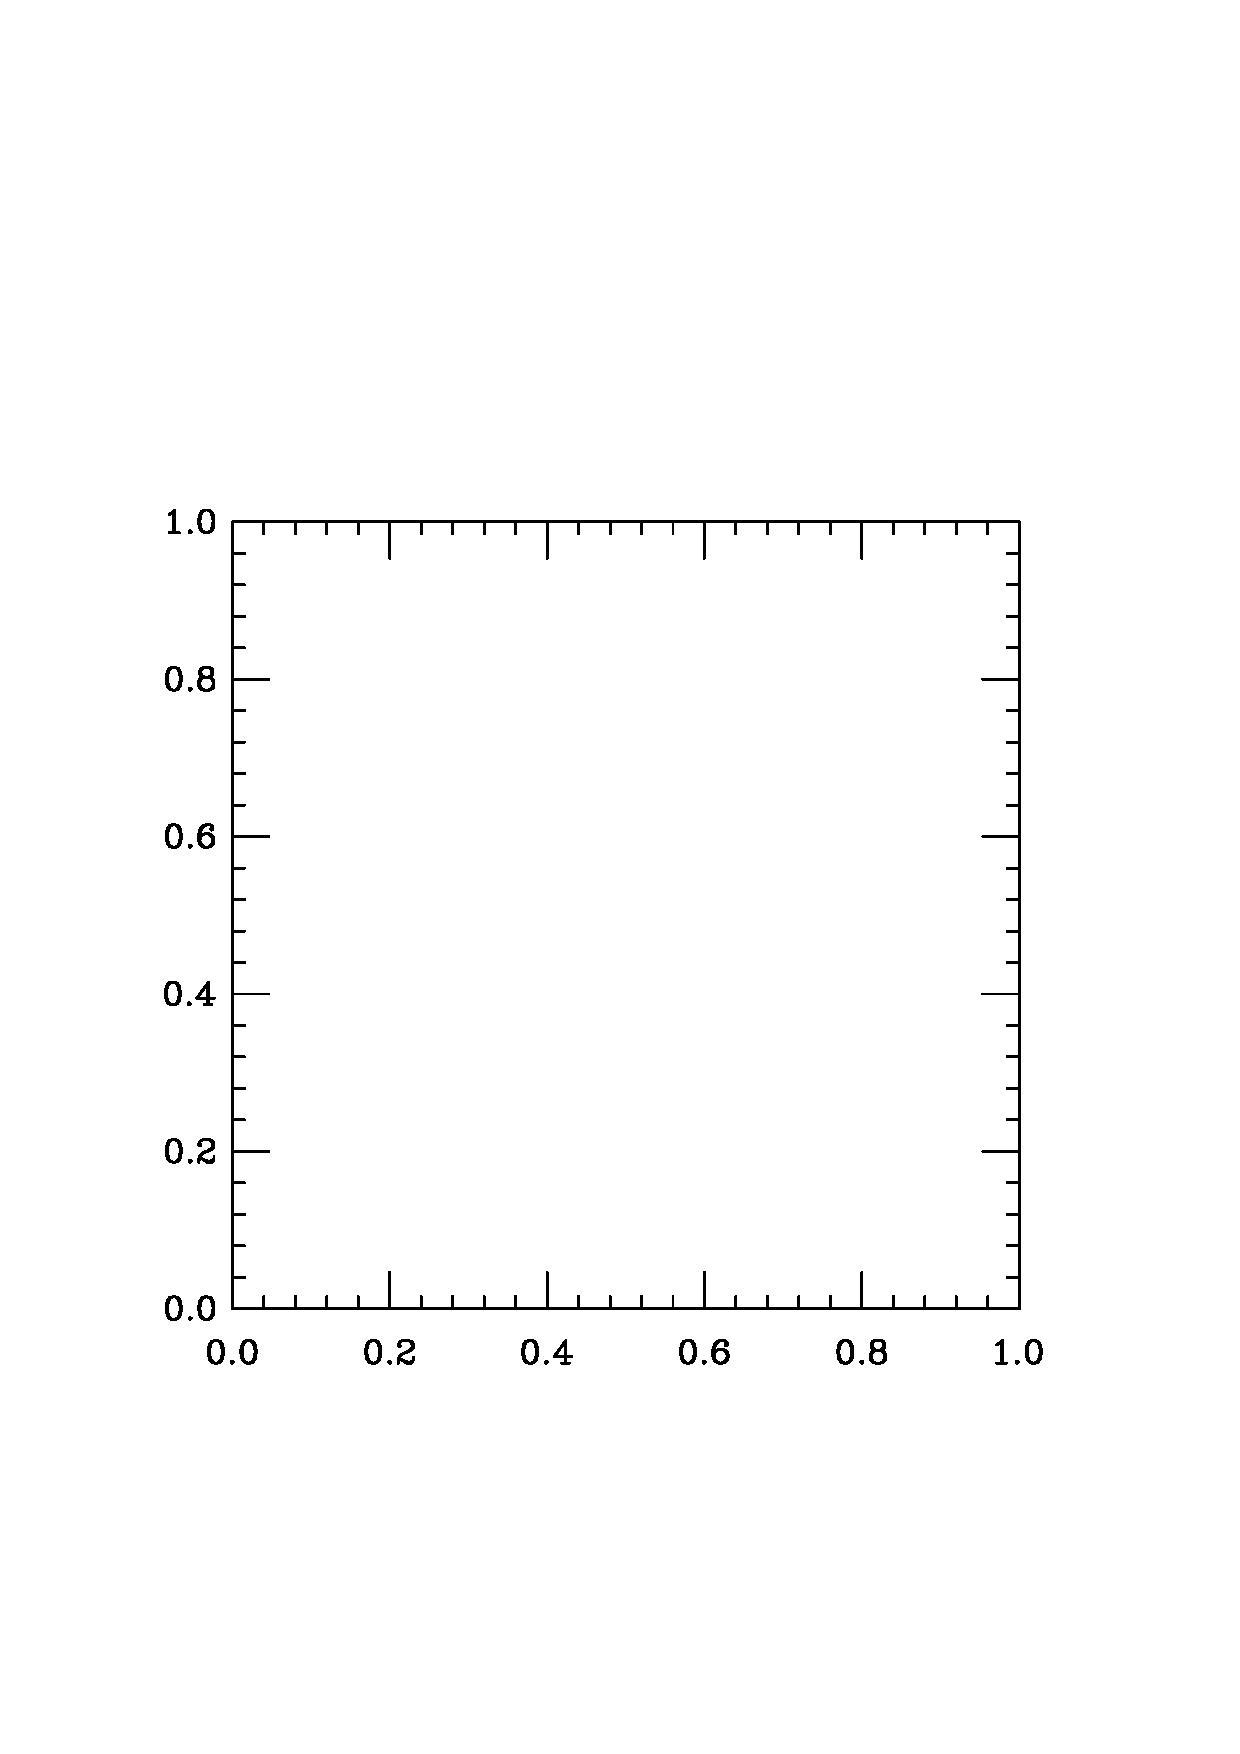
\includegraphics[width=0.8\textwidth]{topsky-crop.pdf}
	\end{center}
\end{minipage}
\begin{minipage}{0.5\textwidth}
	\begin{center}
		\large Sky Below Horizon\\
		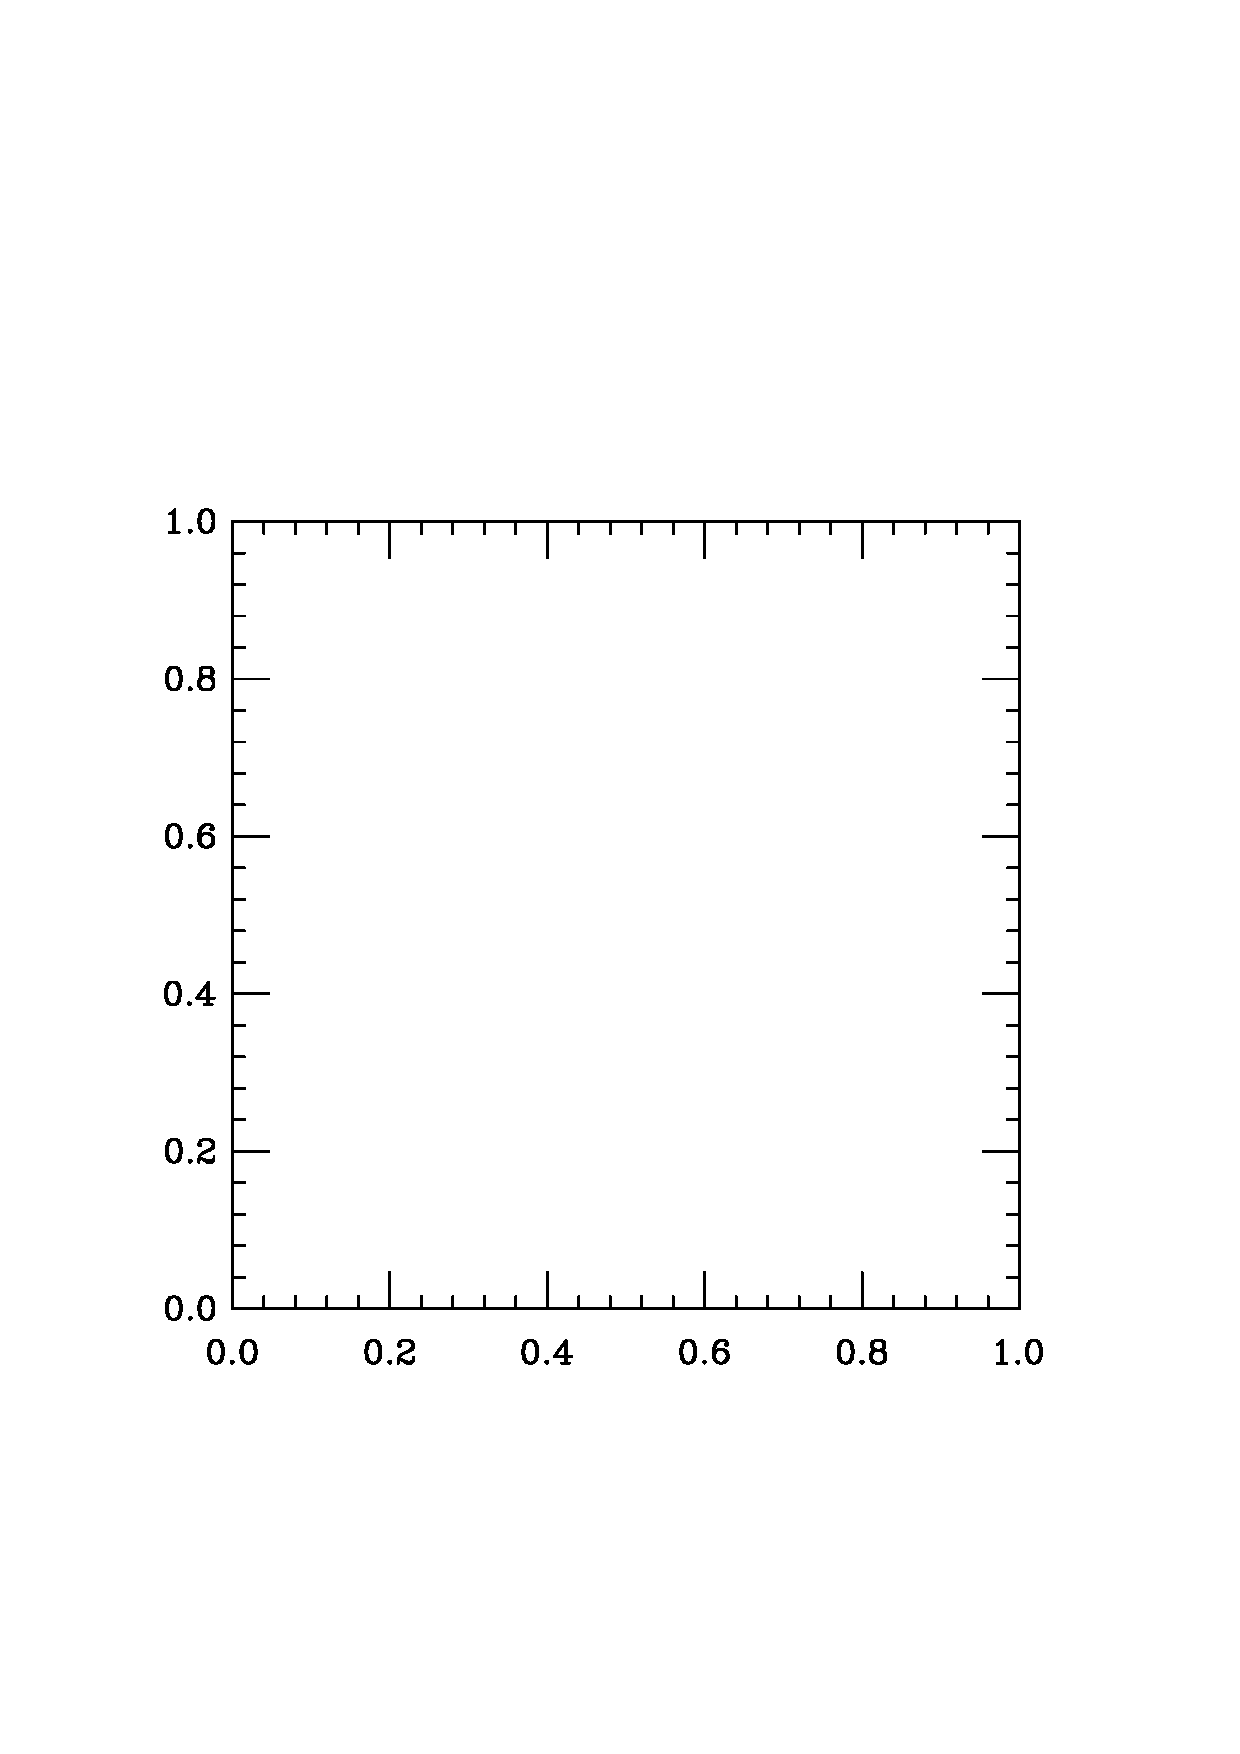
\includegraphics[width=0.8\textwidth]{botsky-crop.pdf}
	\end{center}
\end{minipage}

%
%Look now at the computer animation of the stars rotating on the celestial sphere. There are two stars highlighted on the celestial sphere; we will talk about them later. For now, we need to figure out the relationship between the image shown and the cardinal directions. 
%
%The blue sphere in the middle is the Earth, and the white dot on top is the observer. The red grid (shown) is the observer's {\it horizon}. 
%
%As you know, the horizon has four directions: North, South, East, and West.
%
%\begin{enumerate}
%	\item Which direction (N/S/E/W) is {\it closest to the camera}? How do you know?
%	\insp
%	\item Which direction is to the {\it left} of the image? How do you know?
%	\insp
%	
%	\item Which direction is {\it furthest} from the camera? How do you know?
%	\insp
%	\item Which direction is to the {\it right} of the image? How do you know?
%	\insp
%\end{enumerate}
%
%\subsection{Following the Purple Star}
%
%Stand up in your seat and trace with your finger the path that the purple star takes in your ``sky''. This is the most important part of the entire exercise! 
%
%Four points are labeled on the orbit. It travels from the white dot to the orange dot to the blue dot to the yellow dot, in order.
%
%\begin{enumerate}
%	\item How would you describe the position of the purple star when it is at the {\it white} point on its purple orbit? What star is it below in the sky?
%	
%	\BS\BS\BS
%	
%	\item How would you describe its position at the orange point on its purple orbit?
%	\BS\BS\BS	
%	\item How would you describe its position at the blue point? 
%		\BS\BS\BS
%	\item How would you describe its position at the yellow point?
%		\BS\BS\BS
%		
%		\item Is this star always visible in the observer's sky?
%\end{enumerate}
%
%\subsection{Following the Green Star}
%
%Now, repeat the previous exercise with the green star. This star's motion is close to how the Sun is moving in our sky right now. 
%
%Stand up in your seat and trace with your finger the path that the green star takes in your ``sky''. Again, this is the most important part of this exercise!
%
%Four points are labeled on the orbit. It travels from the white dot to the orange dot to the blue dot to the yellow dot, in order.
%
%\begin{enumerate}
%	\item Which direction would you have to look to see the green star when it is at the {\it orange} point on its orbit? What is that star doing in the sky? (Hint: The Sun does this at about the same time every day.)
%	
%	\BS\BS\BS
%	
%	\item Which way would you look to see the green star when it is at the {\it blue} point in its orbit?
%	\BS\BS\BS	
%	\item Which way would you look to see it at the {\it yellow} point? What is it doing now?
%	\BS\BS\BS
%	\item Which way would you look to see it when it is at the {\it white} point in its orbit?
%	\BS\BS\BS
%\end{enumerate}
%
%\newpage
%
%
%
%\subsection{Drawing the Path of the Purple Star}
%	\begin{minipage}{0.5\textwidth}Here is a depiction of our observer's sky looking North, ``into the page''. Suppose that the purple star is located at the white dot at midnight, low on the northern horizon. 
%	\end{minipage}
%\begin{minipage}{0.5\textwidth}	
%	\begin{center}
%		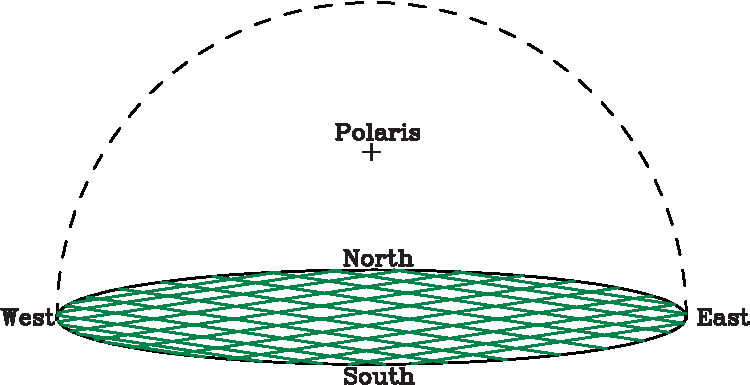
\includegraphics[width=3.5in]{disk-crop.pdf}
%	\end{center}
%		\end{minipage}
%	\begin{enumerate}
%	\item Based on what saw found earlier, draw the path that the purple star will take over {\it one day}. Put arrows on that path showing its direction of motion.
%		\BS
%		
%	\item Where will the purple star be at 6 PM? Label it on your diagram, and describe where you would look in the sky to see it.
%	\insp
%	
%	\item This diagram only shows the observer's northern sky. Could we repeat this exercise and draw the path of the {\it purple} star on the animation here? If you can, do it; if you can't, explain why.
%	
%	\insp \BS\BS
%\end{enumerate}
%
%\newpage

\newpage


\begin{center}
	\sc \Large Astronomy 101 Homework 1 \\ \large The Daily Motion of the Sky -- Due September 8
\end{center}
%\begin{flushright}
%\Large
%
%Name: \underline{\hspace{2.7in}}
%\BS
%
%Lab Section Number: M0\underline{\hspace{1in}}
%\end{flushright}
%
%{\it Instructions: These questions are an extension of the Exercises on the celestial sphere (the first one) and the consequences of the Earth's rotation (the second one). You should tear this page off when you are done so you can turn it in. This is due Thursday, September 9; you will turn them in when you enter the auditorium for class. (We will have a box for you.)}	

\begin{enumerate}
	
	\item Suppose that a star has just risen above the horizon in Syracuse directly to the East. Draw its position on the diagrams below.
	
	
	\begin{minipage}{0.5\textwidth}
		\begin{center}
			\large Sky Above Horizon\\
			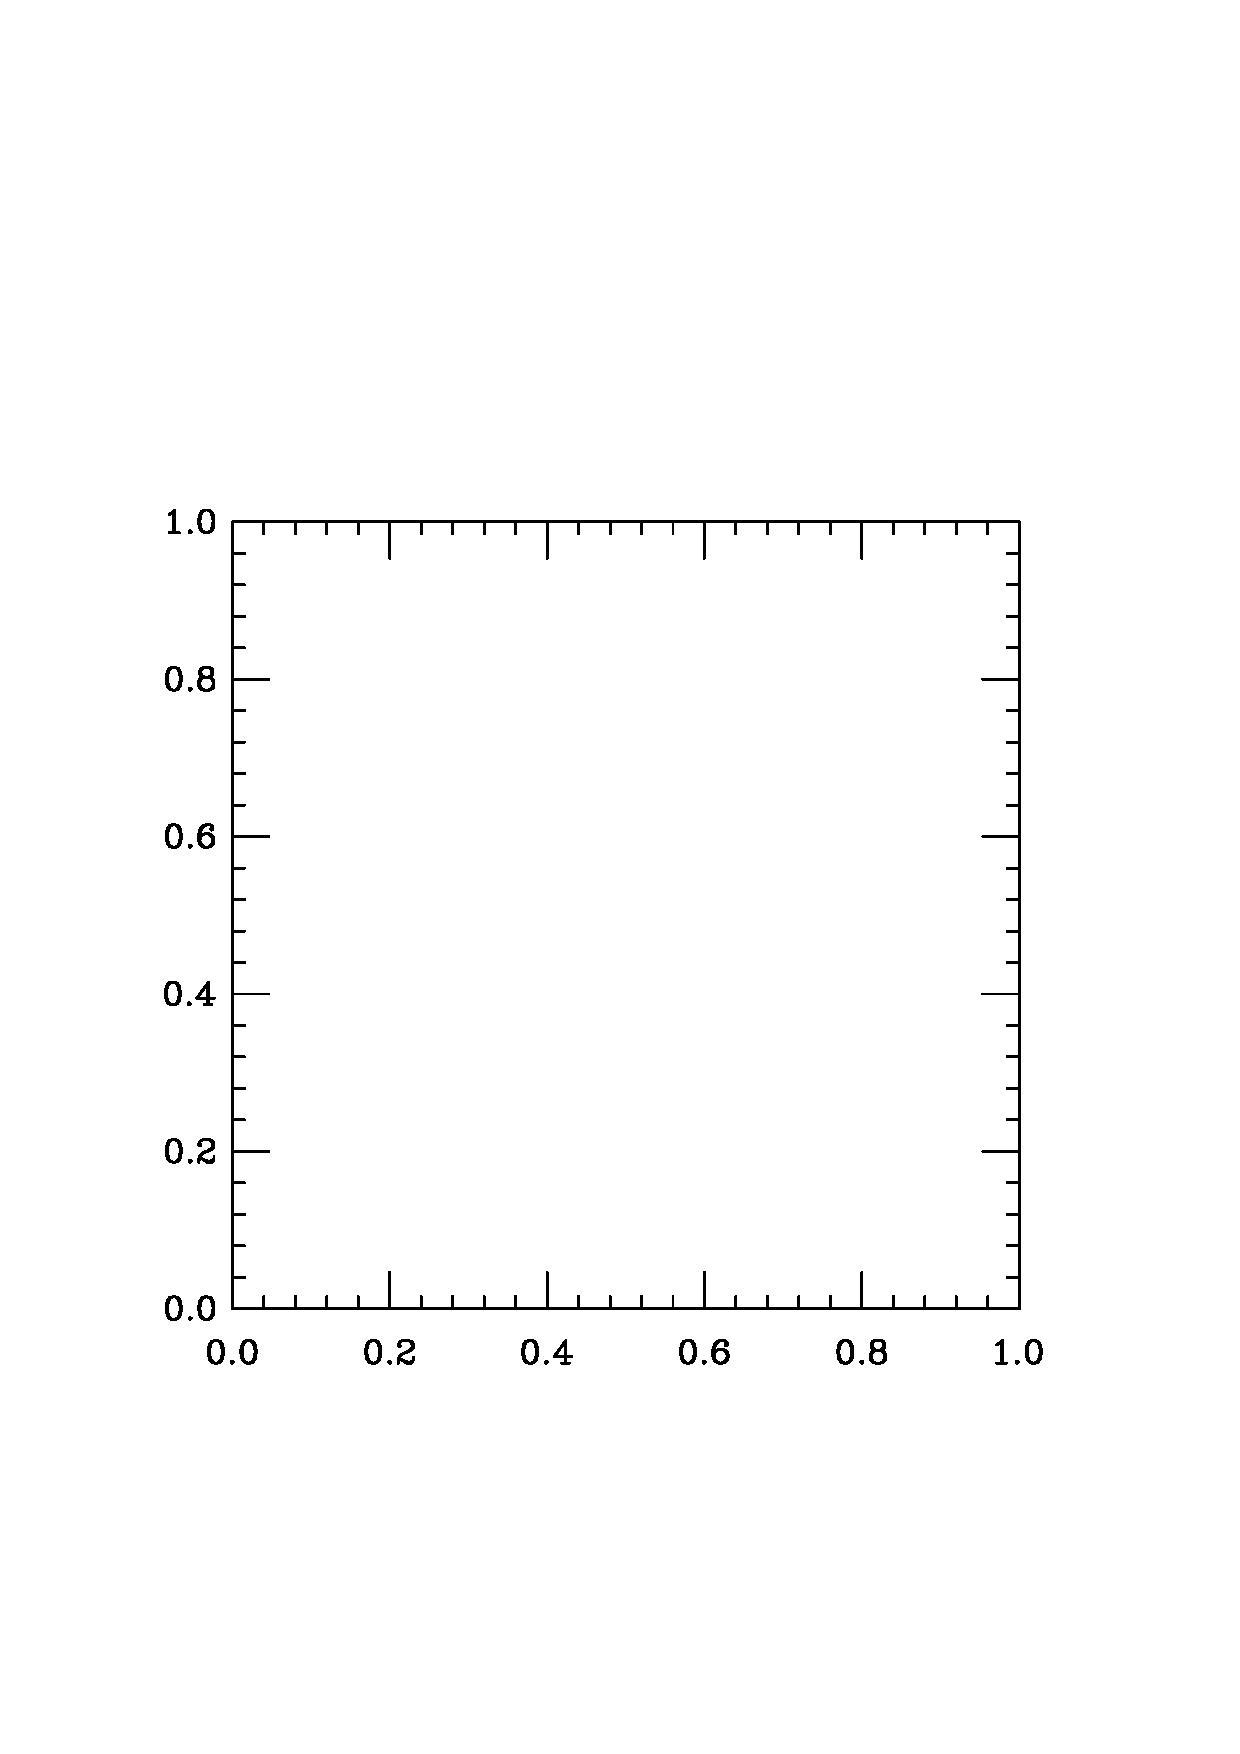
\includegraphics[width=0.8\textwidth]{topsky-crop.pdf}
		\end{center}
	\end{minipage}
	\begin{minipage}{0.5\textwidth}
		\begin{center}
			\large Sky Below Horizon\\
			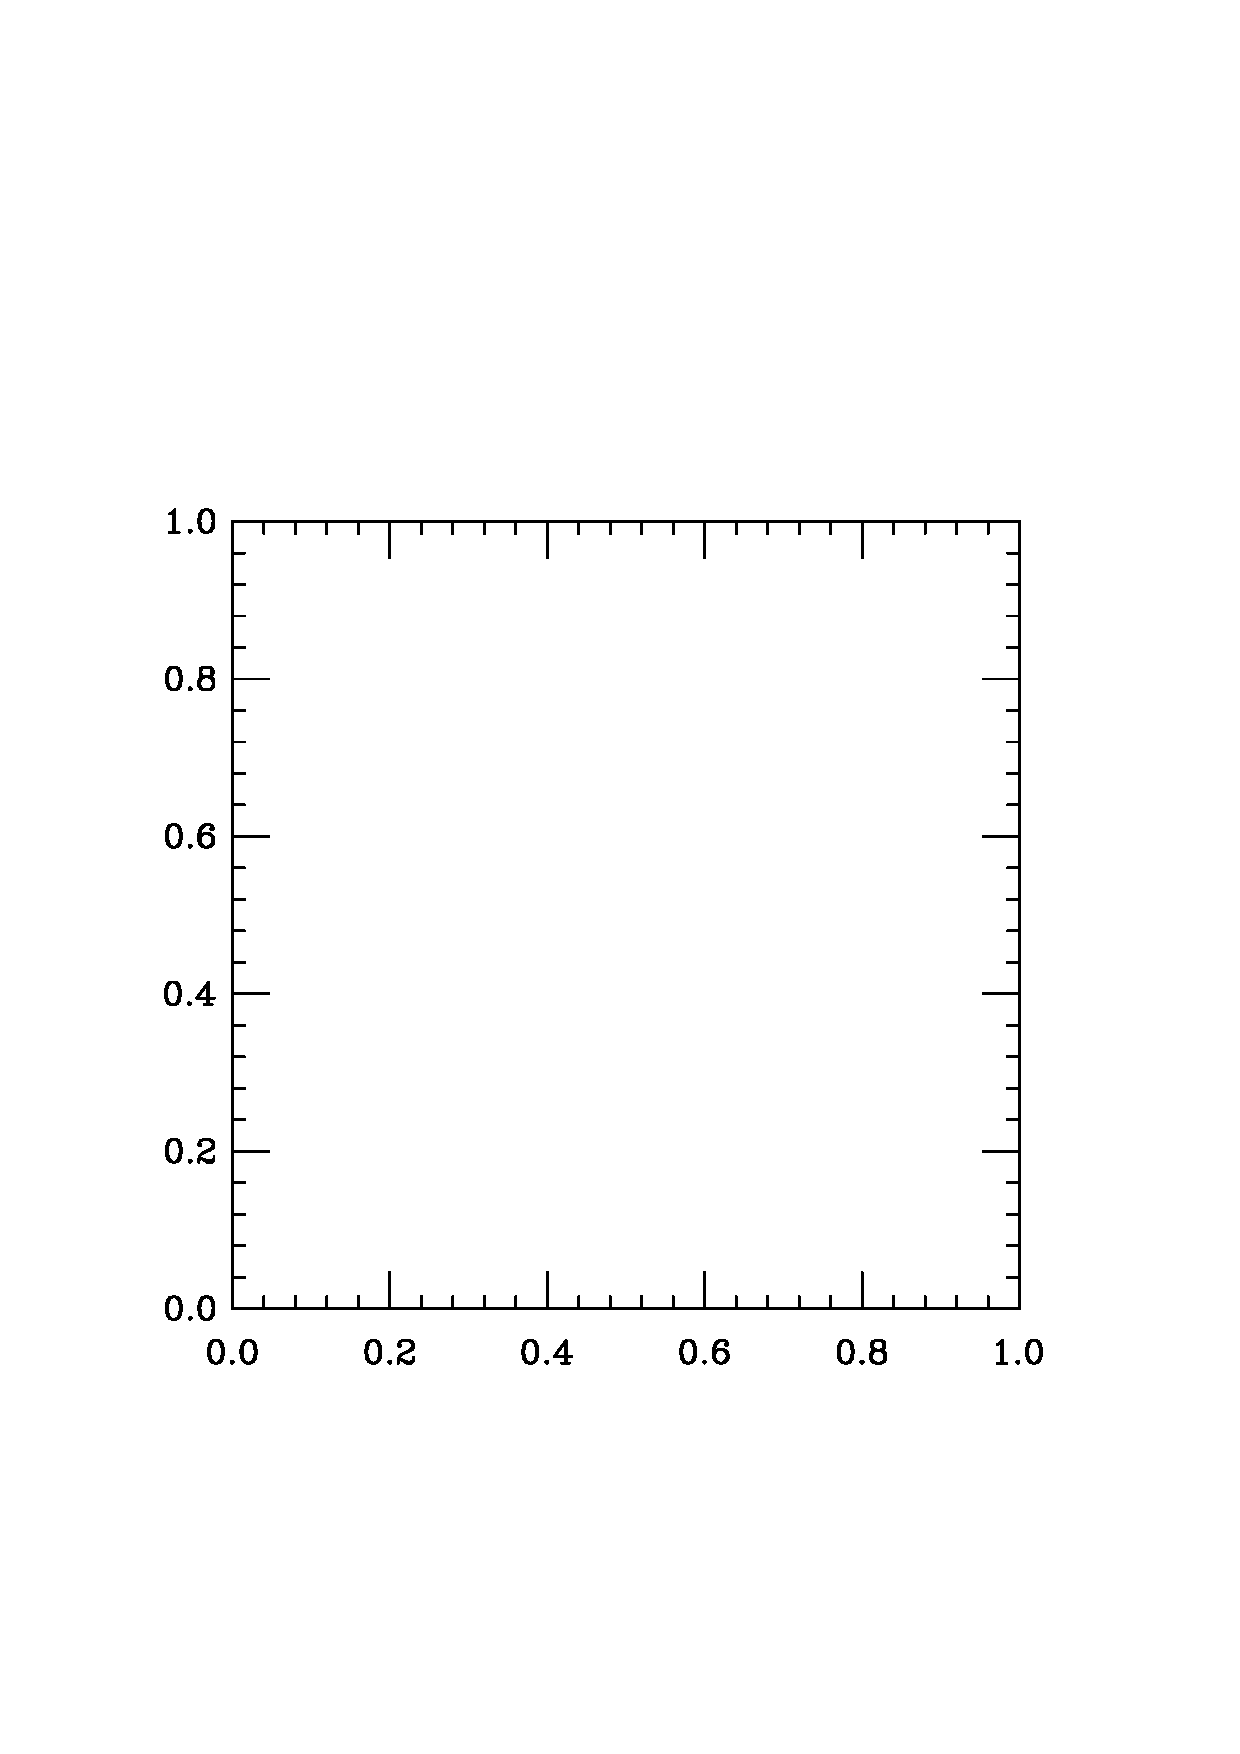
\includegraphics[width=0.8\textwidth]{botsky-crop.pdf}
		\end{center}
	\end{minipage}
	
	\item Describe how it moves after it rises. Does it move straight up in the sky? Does it travel into the southern or northern sky before setting in the west? Draw its path between rising and setting on the diagrams above. Will this star ever reach the zenith?
	
	\insp\bigskip
	

	\item There is also a South Celestial Pole, opposite the North Celestial Pole. As seen from Syracuse, where would it be in the sky? Label it on the diagrams above. Will we ever get to see it?
	
	\insp


   

    \item Describe in words where someone in Alaska, where someone in Ghana, and where someone in New Zealand would see Polaris.
       
    \insp\insp
     \item We know that we can determine which way is north by finding the North Star in the sky. Could someone in Australia find North in the same way? If not, what could they do instead?
 
    
    \insp\bigskip
    
    \item You look up in the sky from Syracuse and see a star high in the northern sky at 6 PM. Draw that star's path on the diagrams below, and label where you expect to find it at midnight and at 6 AM. 
    
	\begin{minipage}{0.5\textwidth}
	\begin{center}
		\large Sky Above Horizon\\
		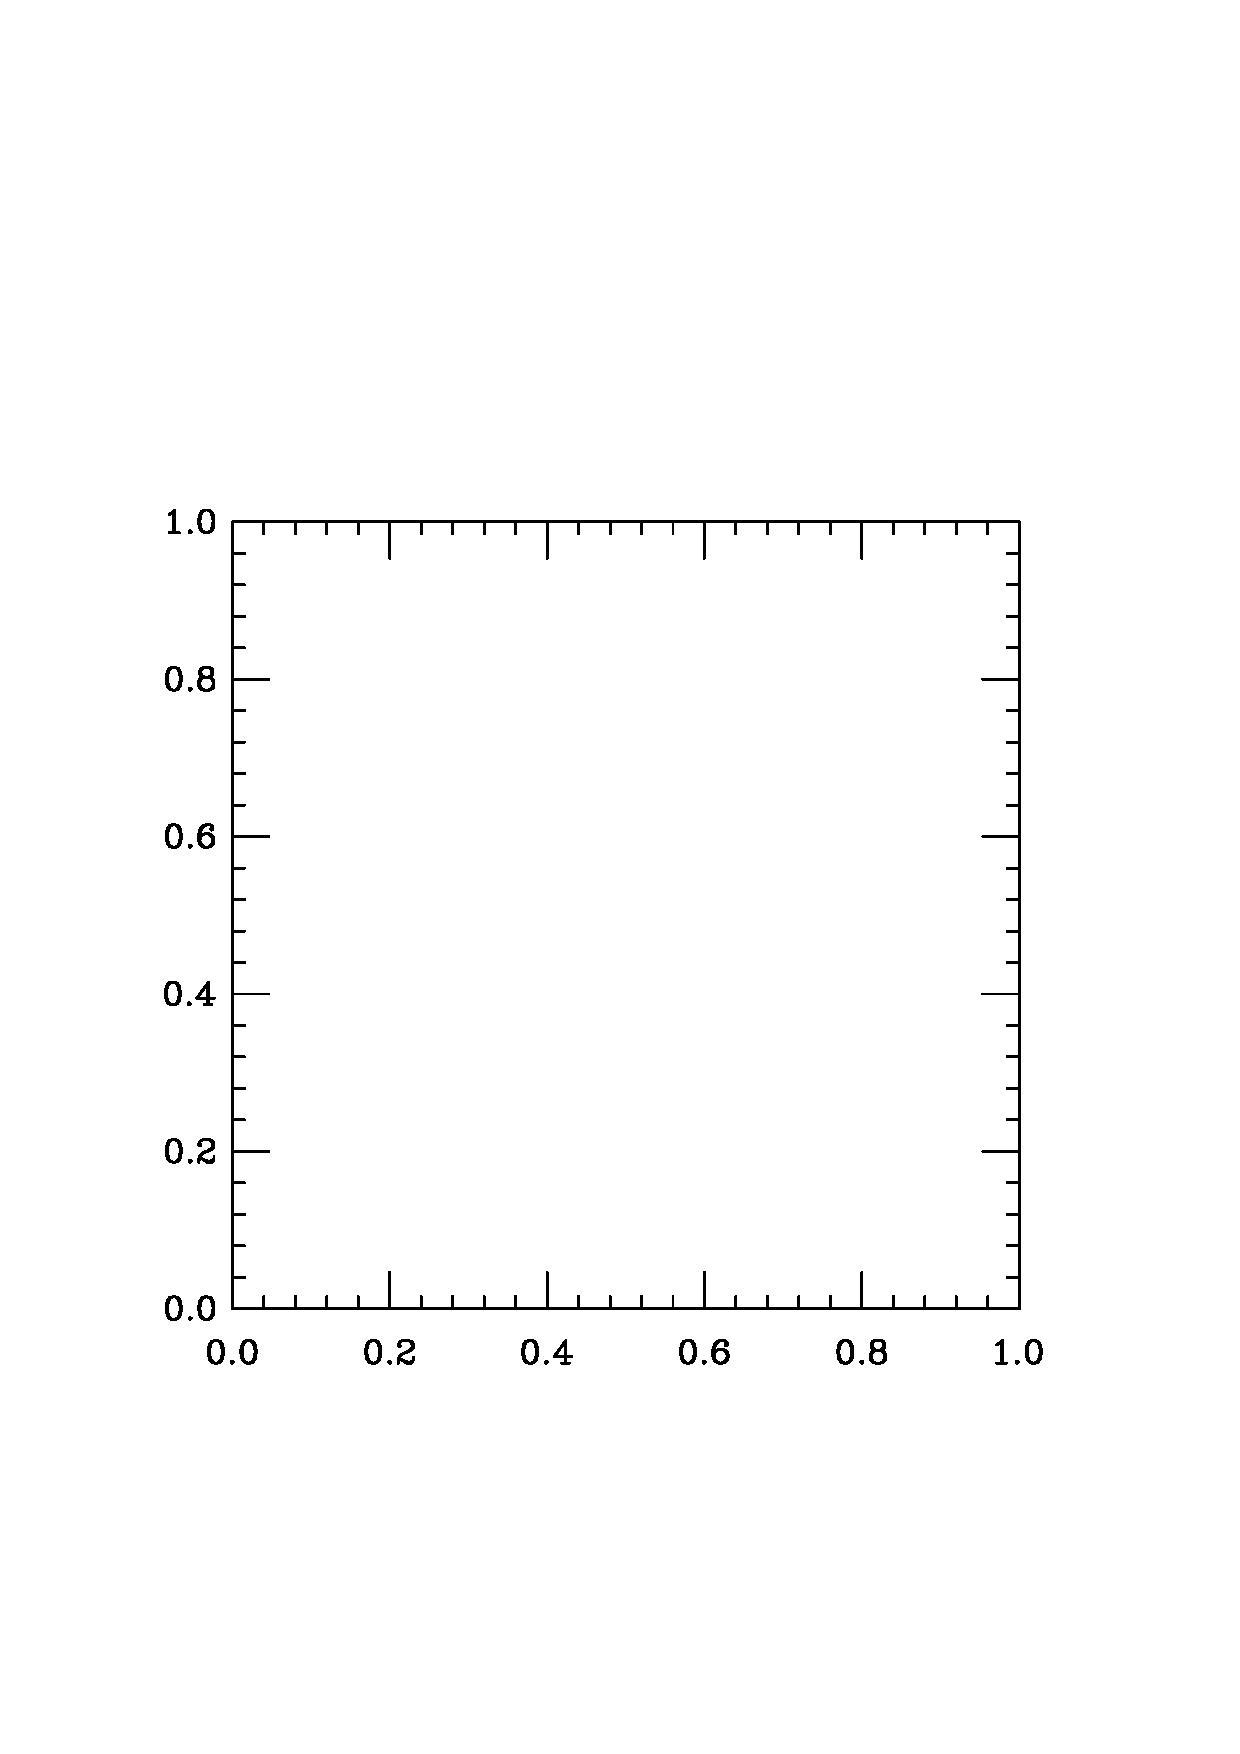
\includegraphics[width=0.8\textwidth]{topsky-crop.pdf}
	\end{center}
\end{minipage}
\begin{minipage}{0.5\textwidth}
	\begin{center}
		\large Sky Below Horizon\\
		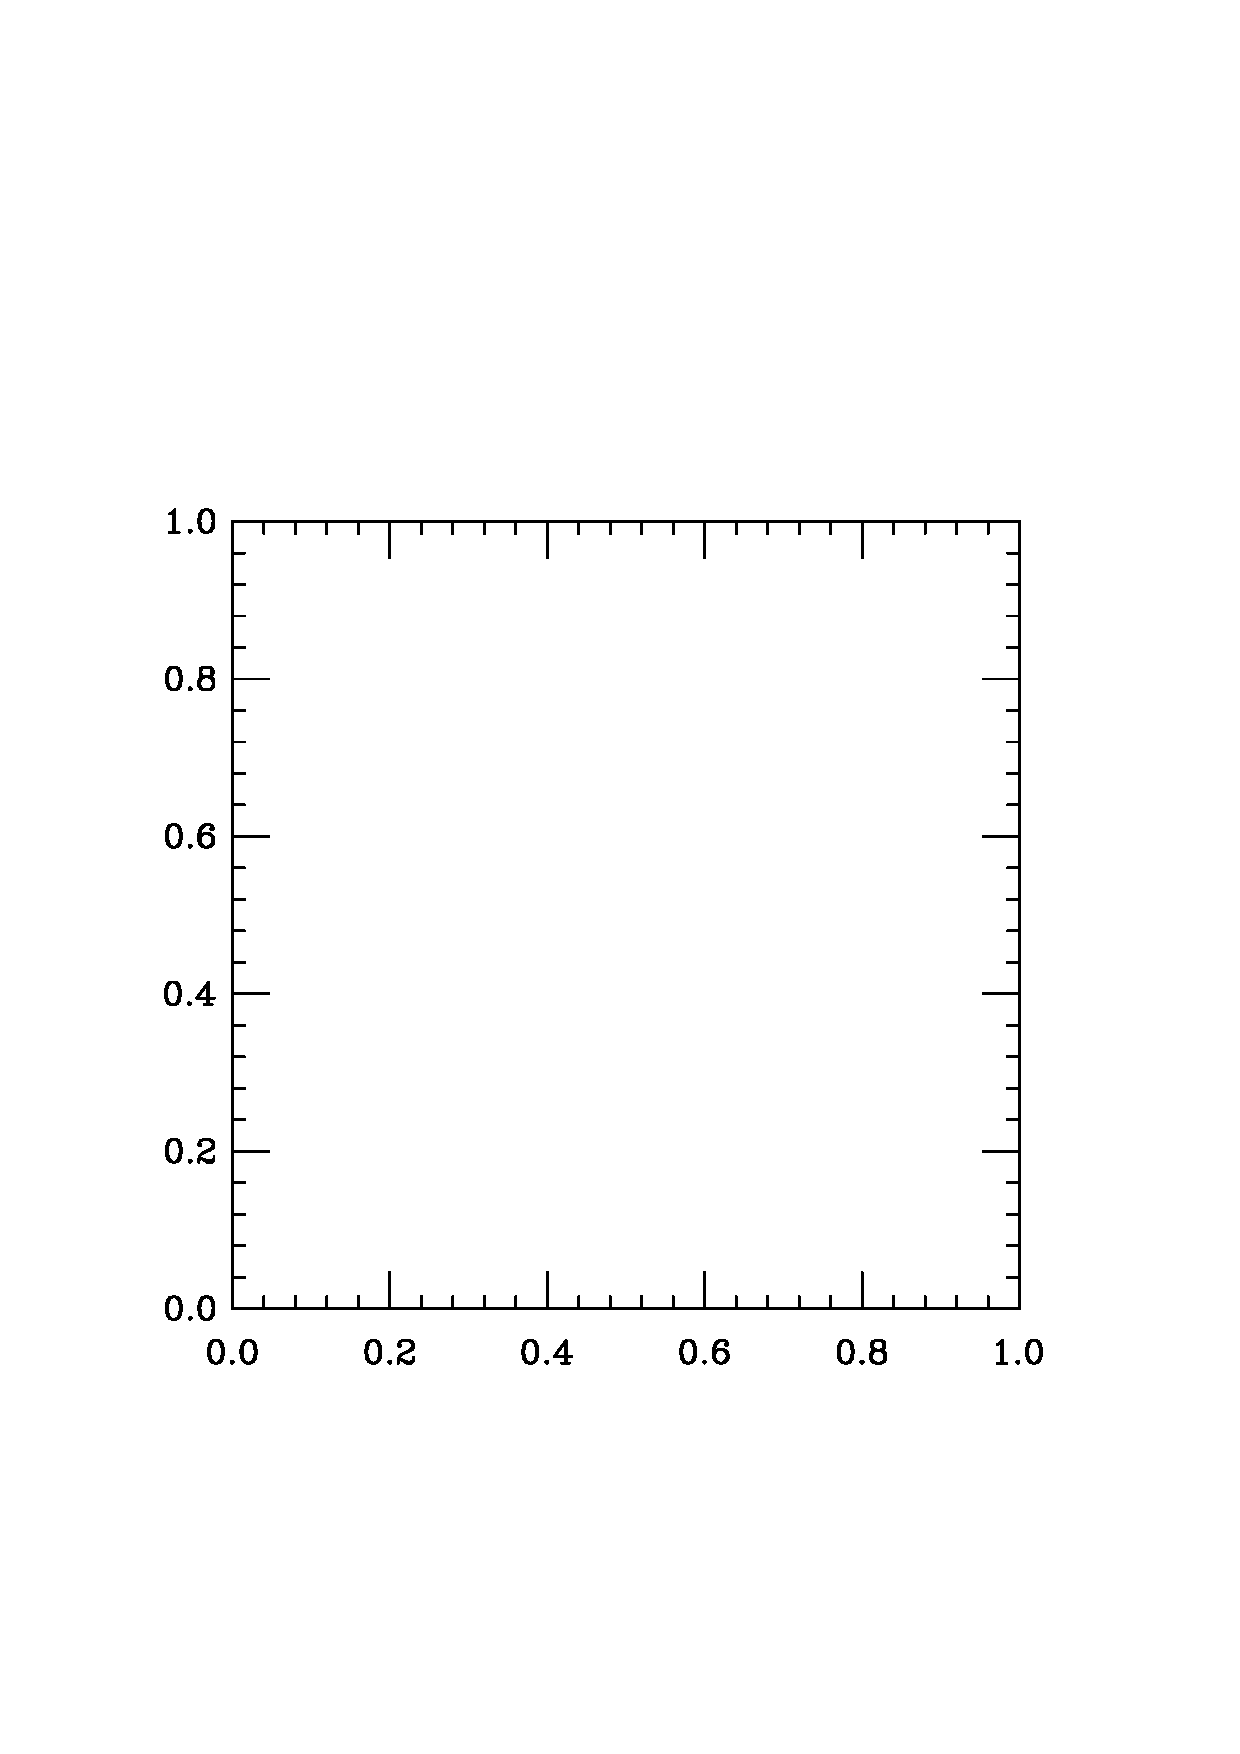
\includegraphics[width=0.8\textwidth]{botsky-crop.pdf}
	\end{center}
\end{minipage}

	\item When will that star set below the horizon? If it will never set, explain how you know this.
	
	\insp\bigskip
	
	{\bf Homework Quiz 1:} This is due September 8. I will not collect it. Instead, you will have a brief homework quiz in class. This homework quiz will have three questions:
	
	\begin{enumerate}
		\item I'll give you the location of a star, either putting it on a diagram or describing it in words, at a certain time of day. Then I will ask you to draw its path for me on a diagram and predict where it will be at a different time of day.
		\item I will ask you to describe where you can find the North and South Celestial Poles from a different location on Earth.
		\item I will describe the motion of a star as seen from Syracuse, and I will ask you how an observer somewhere else on Earth would see it move.
	\end{enumerate}

If you are not sure about how to do these, please come to office hours next Wednesday (room 112, 2-4 PM) and ask before the quiz! You can also go to that room and ask questions during the day; there is almost always a tutor there.
	
\end{enumerate}	

	
\end{document}
	
	
	
	